% Seminar 7: Cointegrare și modele VECM
% Prezentare academică de calitate Harvard
% Program de licență, Academia de Studii Economice din București

\documentclass[9pt, aspectratio=169, t]{beamer}

% Asigură încadrarea conținutului pe diapozitive
\setbeamersize{text margin left=8mm, text margin right=8mm}

%=============================================================================
% CONFIGURARE TEMĂ ȘI STIL
%=============================================================================
\usetheme{default}

% Color Palette (matching Redispatch PDF)
\definecolor{MainBlue}{RGB}{26, 58, 110}
\definecolor{AccentBlue}{RGB}{26, 58, 110}
\definecolor{IDAred}{RGB}{205, 0, 0}
\definecolor{DarkGray}{RGB}{51, 51, 51}
\definecolor{MediumGray}{RGB}{128, 128, 128}
\definecolor{LightGray}{RGB}{248, 248, 248}
\definecolor{VeryLightGray}{RGB}{235, 235, 235}
\definecolor{KeynoteGray}{RGB}{218, 218, 218}
\definecolor{SectionGray}{RGB}{120, 120, 120}
\definecolor{FooterGray}{RGB}{100, 100, 100}
\definecolor{Crimson}{RGB}{220, 53, 69}
\definecolor{Forest}{RGB}{46, 125, 50}
\definecolor{Amber}{RGB}{181, 133, 63}
\definecolor{Orange}{RGB}{230, 126, 34}
\definecolor{Purple}{RGB}{142, 68, 173}

% Gradient background (exact Keynote 315 gradient: white to RGB 218,218,218)
\setbeamertemplate{background}{%
    \begin{tikzpicture}[remember picture, overlay]
        \shade[shading=axis, shading angle=315,
        top color=white, bottom color=KeynoteGray]
        (current page.south west) rectangle (current page.north east);
    \end{tikzpicture}%
}
% Fallback solid color for compatibility
\setbeamercolor{background canvas}{bg=}

\setbeamercolor{palette primary}{bg=MainBlue, fg=white}
\setbeamercolor{palette secondary}{bg=MainBlue!85, fg=white}
\setbeamercolor{palette tertiary}{bg=MainBlue!70, fg=white}
\setbeamercolor{structure}{fg=MainBlue}
\setbeamercolor{title}{fg=IDAred}
\setbeamercolor{frametitle}{fg=IDAred, bg=}
\setbeamercolor{block title}{bg=MainBlue, fg=white}
\setbeamercolor{block body}{bg=VeryLightGray, fg=DarkGray}
\setbeamercolor{block title alerted}{bg=Crimson, fg=white}
\setbeamercolor{block body alerted}{bg=Crimson!8, fg=DarkGray}
\setbeamercolor{block title example}{bg=Forest, fg=white}
\setbeamercolor{block body example}{bg=Forest!8, fg=DarkGray}
\setbeamercolor{item}{fg=MainBlue}

% Footer colors (override Madrid theme blue)
\setbeamercolor{author in head/foot}{fg=FooterGray, bg=}
\setbeamercolor{title in head/foot}{fg=FooterGray, bg=}
\setbeamercolor{date in head/foot}{fg=FooterGray, bg=}
\setbeamercolor{section in head/foot}{fg=FooterGray, bg=}
\setbeamercolor{subsection in head/foot}{fg=FooterGray, bg=}

% Bullet styles (apply everywhere including blocks)
\setbeamertemplate{itemize item}{\color{MainBlue}$\boxdot$}
\setbeamertemplate{itemize subitem}{\color{MainBlue}$\blacktriangleright$}
\setbeamertemplate{itemize subsubitem}{\color{MainBlue}\tiny$\bullet$}
\setbeamertemplate{itemize/enumerate body begin}{\normalsize}
\setbeamertemplate{itemize/enumerate subbody begin}{\normalsize}

% Item spacing - compact style
\setlength{\leftmargini}{10pt}       % Level 1: minimal indent
\setlength{\leftmarginii}{10pt}      % Level 2: minimal additional indent
% Compact list spacing (zero extra space before/after lists in blocks)
\makeatletter
\def\@listi{\leftmargin\leftmargini \topsep 0pt \parsep 0pt \itemsep 0pt}
\def\@listii{\leftmargin\leftmarginii \topsep 0pt \parsep 0pt \itemsep 0pt}
\makeatother

\setbeamertemplate{navigation symbols}{}

%=============================================================================
% CUSTOM HEADLINE
%=============================================================================
\setbeamertemplate{headline}{%
    \vskip10pt%
    \hbox to \paperwidth{%
        \hskip0.5cm%
        {\small\color{FooterGray}\renewcommand{\hyperlink}[2]{##2}\insertsectionhead}%
        \hfill%
        \textcolor{FooterGray}{\small\insertframenumber}%
        \hskip0.5cm%
    }%
    \vskip4pt%
    {\color{FooterGray}\hrule height 0.4pt}%
}

%=============================================================================
% CUSTOM FOOTER
%=============================================================================
\usepackage{fontawesome5}

\setbeamertemplate{footline}{%
    {\color{FooterGray}\hrule height 0.4pt}%
    \vskip4pt%
    \hbox to \paperwidth{%
        \hskip0.5cm%
        \textcolor{FooterGray}{\small Analiza și Prognoza seriilor de timp}%
        \hfill%
        \raisebox{-0.1em}{%
            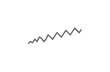
\begin{tikzpicture}[x=0.08em, y=0.08em, line width=0.4pt]
                \draw[FooterGray] (0,3) -- (1,4) -- (2,3.5) -- (3,5) -- (4,4) -- (5,6) -- (6,5.5) -- (7,4) -- (8,5) -- (9,7) -- (10,6) -- (11,5) -- (12,6.5) -- (13,8) -- (14,7) -- (15,6) -- (16,7.5) -- (17,9) -- (18,8) -- (19,7) -- (20,8.5) -- (21,10) -- (22,9) -- (23,8) -- (24,9.5);
            \end{tikzpicture}%
        }%
        \hskip0.5cm%
    }%
    \vskip6pt%
}

%=============================================================================
% PACHETE
%=============================================================================
\usepackage[utf8]{inputenc}
\usepackage[T1]{fontenc}
\usepackage[romanian]{babel}
\usepackage{amsmath, amssymb, amsthm}
\usepackage{mathtools}
\usepackage{bm}
\usepackage{tikz}
\usetikzlibrary{arrows.meta, positioning, shapes, calc, decorations.pathreplacing, shadings}
\usepackage{booktabs}
\usepackage{multirow}
\usepackage{array}
\usepackage{graphicx}
\usepackage{hyperref}
\usepackage{colortbl}
\hypersetup{colorlinks=true, linkcolor=MainBlue, urlcolor=MainBlue}
\graphicspath{{../../logos/}{../../charts/}}
\hfuzz=2pt  % Suppress tiny overfull warnings (<2pt)
\vfuzz=2pt  % Suppress tiny vertical overfull warnings (<2pt)

%=============================================================================
% COMANDA QUANTLET
%=============================================================================
\newcommand{\quantlet}[2]{%
    \hfill\href{#2}{%
        \raisebox{-0.15em}{\includegraphics[height=0.7em]{ql_logo.png}}%
        \textcolor{MainBlue}{\tiny\ #1}%
    }%
}

%=============================================================================
% COMENZI PERSONALIZATE
%=============================================================================
\newcommand{\E}{\mathbb{E}}
\newcommand{\Var}{\text{Var}}
\newcommand{\Cov}{\text{Cov}}
\newcommand{\Corr}{\text{Corr}}
\newcommand{\R}{\mathbb{R}}
\newcommand{\RMSE}{\text{RMSE}}
\newcommand{\MAE}{\text{MAE}}
\newcommand{\MAPE}{\text{MAPE}}
% Bold math commands for VECM models
\newcommand{\bY}{\mathbf{Y}}
\newcommand{\bX}{\mathbf{X}}
\newcommand{\bPi}{\boldsymbol{\Pi}}
\newcommand{\balpha}{\boldsymbol{\alpha}}
\newcommand{\bbeta}{\boldsymbol{\beta}}
\newcommand{\bGamma}{\boldsymbol{\Gamma}}
\newcommand{\bvarepsilon}{\boldsymbol{\varepsilon}}
\newcommand{\bepsilon}{\boldsymbol{\varepsilon}}
\newcommand{\bc}{\mathbf{c}}

\newcommand{\correct}{\textcolor{Forest}{\checkmark}}
\newcommand{\incorrect}{\textcolor{Crimson}{\texttimes}}

%=============================================================================
% PAGINA TITLU PERSONALIZATA
%=============================================================================
\defbeamertemplate*{title page}{hybrid}[1][]
{
    \vspace{0.2cm}
    \begin{center}
        \href{https://www.ase.ro}{\includegraphics[height=1.0cm]{ase_logo.png}}\hspace{0.3cm}%
        \href{https://theida.net}{\includegraphics[height=1.0cm]{ida_logo.png}}\hspace{0.3cm}%
        \href{https://blockchain-research-center.com}{\includegraphics[height=1.0cm]{brc_logo.png}}\hspace{0.3cm}%
        \href{https://www.ai4efin.ase.ro}{\includegraphics[height=1.0cm]{ai4efin_logo.png}}\hspace{0.3cm}%
        \href{https://ipe.ro/new}{\includegraphics[height=1.0cm]{acad_logo.png}}\hspace{0.3cm}%
        \href{https://www.digital-finance-msca.com}{\includegraphics[height=1.0cm]{msca_logo.png}}%
    \end{center}

    \vspace{0.6cm}

    \begin{center}
        \begin{minipage}{0.1\textwidth}
            \centering
            \href{https://quantlet.com}{\includegraphics[height=1.1cm]{ql_logo.png}}
        \end{minipage}%
        \begin{minipage}{0.78\textwidth}
            \centering
            {\LARGE\bfseries\usebeamercolor[fg]{title}\inserttitle}

            \vspace{0.3cm}

            {\usebeamerfont{subtitle}\usebeamercolor[fg]{title}\insertsubtitle}
        \end{minipage}%
        \begin{minipage}{0.1\textwidth}
            \centering
            \href{https://quantinar.com}{\includegraphics[height=1.1cm]{qr_logo.png}}
        \end{minipage}
    \end{center}

    \vspace{0.6cm}

    \hspace{0.5cm}{\usebeamerfont{author}\insertauthor}

    \vspace{0.3cm}

    \hspace{0.5cm}\begin{minipage}[t]{0.9\textwidth}
        \raggedright\small\insertinstitute
    \end{minipage}
}

%=============================================================================
% INFORMATII TITLU
%=============================================================================
\title[Analiza Seriilor de Timp]{Analiza și Prognoza seriilor de timp}
\subtitle{Seminar 7: Cointegrare și modele VECM}
\author[D.T. Pele]{Daniel Traian PELE}
\institute{Academia de Studii Economice din București\\
IDA Institute Digital Assets\\
Blockchain Research Center\\
AI4EFin Artificial Intelligence for Energy Finance\\
Academia Română, Institutul de Prognoză Economică\\
MSCA Digital Finance}
\date{}

\begin{document}

% Title page (no header/footer)
{
\setbeamertemplate{headline}{}
\setbeamertemplate{footline}{}
\begin{frame}
    \titlepage
\end{frame}
}

%=============================================================================
% OUTLINE
%=============================================================================
\begin{frame}{Cuprins Seminar}
    \tableofcontents
\end{frame}

%=============================================================================
% SECTION 1: REVIEW QUIZ
%=============================================================================
\section{Test de Recapitulare}

\begin{frame}{Test 1: Definiția Cointegrării}
    \begin{alertblock}{Întrebare}
        Două variabile I(1), $X_t$ și $Y_t$, sunt cointegrate dacă:
    \end{alertblock}

    \vspace{0.3cm}

    \begin{block}{Variante de răspuns}
        \textcolor{MainBlue}{\textbf{(A)}} Ambele sunt staționare\\[3pt]
        \textcolor{MainBlue}{\textbf{(B)}} Suma lor este I(2)\\[3pt]
        \textcolor{MainBlue}{\textbf{(C)}} O combinație liniară a lor este I(0)\\[3pt]
        \textcolor{MainBlue}{\textbf{(D)}} Au aceeași medie
    \end{block}

    \vspace{0.5cm}
    \begin{flushright}\textit{Răspunsul pe slide-ul următor...}\end{flushright}
\end{frame}

\begin{frame}{Test 1: Răspuns}
    \begin{exampleblock}{Răspuns: C -- O combinație liniară este I(0)}
        \begin{center}
            \includegraphics[width=0.85\textwidth, height=0.60\textheight, keepaspectratio]{ch6_quiz1_cointegration.pdf}
        \end{center}
        \vspace{-0.2cm}
        {\footnotesize
        \textbf{Cheie}: $Y_t - \beta X_t \sim I(0)$ înseamnă că seriile au un trend stochastic comun. Combinația liniară (spread-ul) este staționară chiar dacă ambele serii sunt nestaționare.
        }
    \end{exampleblock}
\end{frame}

\begin{frame}{Test 2: Regresia falsă}
    \begin{alertblock}{Întrebare}
        Când regresăm un mers aleator pe alt mers aleator independent, de obicei obținem:
    \end{alertblock}

    \vspace{0.3cm}

    \begin{block}{Variante de răspuns}
        \textcolor{MainBlue}{\textbf{(A)}} $R^2$ mic și coeficienți nesemnificativi\\[3pt]
        \textcolor{MainBlue}{\textbf{(B)}} $R^2$ mare și coeficienți semnificativi (fals!)\\[3pt]
        \textcolor{MainBlue}{\textbf{(C)}} Coeficienți zero\\[3pt]
        \textcolor{MainBlue}{\textbf{(D)}} Rezultate nedefinite
    \end{block}

    \vspace{0.5cm}
    \begin{flushright}\textit{Răspunsul pe slide-ul următor...}\end{flushright}
\end{frame}

\begin{frame}{Test 2: Răspuns}
    \begin{exampleblock}{Răspuns: B -- $R^2$ mare și coeficienți semnificativi (fals!)}
        \begin{center}
            \includegraphics[width=0.85\textwidth, height=0.60\textheight, keepaspectratio]{ch6_quiz2_spurious.pdf}
        \end{center}
        \vspace{-0.2cm}
        {\footnotesize
        \textbf{Granger-Newbold (1974)}: Regresarea seriilor I(1) nerelaționate dă rezultate înșelătoare. Regulă: Dacă $R^2 > DW$, suspectați regresie falsă!
        \faIcon{globe} Exemple reale: \href{https://www.tylervigen.com/spurious-correlations}{\texttt{tylervigen.com/spurious-correlations}}
        }
    \end{exampleblock}
\end{frame}

\begin{frame}{Test 3: Testul Engle-Granger}
    \begin{alertblock}{Întrebare}
        În metoda Engle-Granger în doi pași, ce testăm în pasul 2?
    \end{alertblock}

    \vspace{0.3cm}

    \begin{block}{Variante de răspuns}
        \textcolor{MainBlue}{\textbf{(A)}} Dacă variabilele originale sunt staționare\\[3pt]
        \textcolor{MainBlue}{\textbf{(B)}} Dacă reziduurile regresiei au rădăcină unitară\\[3pt]
        \textcolor{MainBlue}{\textbf{(C)}} Dacă coeficienții sunt semnificativi\\[3pt]
        \textcolor{MainBlue}{\textbf{(D)}} Dacă $R^2$ este suficient de mare
    \end{block}

    \vspace{0.5cm}
    \begin{flushright}\textit{Răspunsul pe slide-ul următor...}\end{flushright}
\end{frame}

\begin{frame}{Test 3: Răspuns}
    \begin{exampleblock}{Răspuns: B -- Dacă reziduurile au rădăcină unitară}
        \textbf{Pasul 1}: Rulăm OLS: $Y_t = \alpha + \beta X_t + e_t$, salvăm reziduurile $\hat{e}_t$

        \vspace{0.2cm}
        \textbf{Pasul 2}: Test ADF pe reziduuri: $\Delta \hat{e}_t = \rho \hat{e}_{t-1} + \ldots$
        \begin{itemize}
            \item $H_0$: $\rho = 0$ (rădăcină unitară $\Rightarrow$ fără cointegrare)
            \item $H_1$: $\rho < 0$ (staționar $\Rightarrow$ cointegrare!)
        \end{itemize}

        \vspace{0.2cm}
        \textbf{Important}: Folosiți valorile critice Engle-Granger, nu ADF standard!
    \end{exampleblock}
\end{frame}

\begin{frame}{Test 4: Avantajul Testului Johansen}
    \begin{alertblock}{Întrebare}
        Principalul avantaj al testului Johansen față de Engle-Granger este:
    \end{alertblock}

    \vspace{0.3cm}

    \begin{block}{Variante de răspuns}
        \textcolor{MainBlue}{\textbf{(A)}} Este mai simplu de calculat\\[3pt]
        \textcolor{MainBlue}{\textbf{(B)}} Poate detecta relații de cointegrare multiple\\[3pt]
        \textcolor{MainBlue}{\textbf{(C)}} Nu necesită date\\[3pt]
        \textcolor{MainBlue}{\textbf{(D)}} Găsește întotdeauna cointegrare
    \end{block}

    \vspace{0.5cm}
    \begin{flushright}\textit{Răspunsul pe slide-ul următor...}\end{flushright}
\end{frame}

\begin{frame}{Test 4: Răspuns}
    \vspace{0.3cm}
    \begin{center}
        \includegraphics[width=0.75\textwidth, height=0.38\textheight, keepaspectratio]{ch6_quiz4_johansen.pdf}
    \end{center}
    \vspace{-0.1cm}
    \begin{block}{Observații}
    {\small
        \begin{itemize}\setlength{\itemsep}{2pt}
            \item Testează pentru $r = 0, 1, 2, \ldots, k-1$ vectori de cointegrare
            \item Verosimilitate maximă (mai eficient)
            \item Nu necesită alegerea variabilei dependente
        \end{itemize}
    }
    \end{block}
\end{frame}

\begin{frame}{Test 5: Rangul Matricei $\bPi$}
    \begin{alertblock}{Întrebare}
        Într-un VECM cu $k=3$ variabile, dacă $\text{rang}(\bPi) = 2$, aceasta înseamnă:
    \end{alertblock}

    \vspace{0.3cm}

    \begin{block}{Variante de răspuns}
        \textcolor{MainBlue}{\textbf{(A)}} Fără cointegrare\\[3pt]
        \textcolor{MainBlue}{\textbf{(B)}} O relație de cointegrare\\[3pt]
        \textcolor{MainBlue}{\textbf{(C)}} Două relații de cointegrare\\[3pt]
        \textcolor{MainBlue}{\textbf{(D)}} Toate variabilele sunt staționare
    \end{block}

    \vspace{0.5cm}
    \begin{flushright}\textit{Răspunsul pe slide-ul următor...}\end{flushright}
\end{frame}

\begin{frame}{Test 5: Răspuns}
    \begin{exampleblock}{Răspuns: C -- Două relații de cointegrare}
        \textbf{Interpretarea rangului} pentru $k$ variabile:
        \begin{itemize}
            \item $\text{rang}(\bPi) = 0$: Fără cointegrare (folosiți VAR în diferențe)
            \item $0 < \text{rang}(\bPi) = r < k$: $r$ vectori de cointegrare (folosiți VECM)
            \item $\text{rang}(\bPi) = k$: Toate variabilele sunt I(0) (folosiți VAR în niveluri)
        \end{itemize}

        \vspace{0.2cm}
        \textbf{Cu $k=3$ și $r=2$}:
        \begin{itemize}
            \item Două relații de echilibru
            \item Doar $k - r = 1$ trend stochastic comun
        \end{itemize}
    \end{exampleblock}
\end{frame}

\begin{frame}{Test 6: Structura VECM}
    \begin{alertblock}{Întrebare}
        În ecuația VECM $\Delta \bY_t = \bc + \balpha\bbeta'\bY_{t-1} + \ldots$, ce reprezintă $\balpha$?
    \end{alertblock}

    \vspace{0.3cm}

    \begin{block}{Variante de răspuns}
        \textcolor{MainBlue}{\textbf{(A)}} Vectorii de cointegrare\\[3pt]
        \textcolor{MainBlue}{\textbf{(B)}} Coeficienții de ajustare (încărcare)\\[3pt]
        \textcolor{MainBlue}{\textbf{(C)}} Dinamica pe termen scurt\\[3pt]
        \textcolor{MainBlue}{\textbf{(D)}} Varianța erorilor
    \end{block}

    \vspace{0.5cm}
    \begin{flushright}\textit{Răspunsul pe slide-ul următor...}\end{flushright}
\end{frame}

\begin{frame}{Test 6: Răspuns}
    \vspace{0.3cm}
    \begin{center}
        \includegraphics[width=0.75\textwidth, height=0.38\textheight, keepaspectratio]{ch6_quiz6_adjustment.pdf}
    \end{center}
    \vspace{-0.1cm}
    \begin{block}{Observații}
    {\small
        \begin{itemize}\setlength{\itemsep}{2pt}
            \item $\bbeta$ = vectorii de cointegrare (definesc echilibrul)
            \item $\balpha$ = vitezele de ajustare (cât de repede corectează fiecare variabilă)
        \end{itemize}
    }
    \end{block}
\end{frame}

\begin{frame}{Test 7: Termenul de Corecție a Erorilor}
    \begin{alertblock}{Întrebare}
        Dacă $Y_t - \beta X_t$ este relația de cointegrare și acest termen este pozitiv, ce se întâmplă?
    \end{alertblock}

    \vspace{0.3cm}

    \begin{block}{Variante de răspuns}
        \textcolor{MainBlue}{\textbf{(A)}} $Y$ este deasupra echilibrului; $Y$ ar trebui să scadă (dacă $\alpha < 0$)\\[3pt]
        \textcolor{MainBlue}{\textbf{(B)}} $Y$ este sub echilibru; $Y$ ar trebui să crească\\[3pt]
        \textcolor{MainBlue}{\textbf{(C)}} Nimic, corecția erorilor nu afectează nivelurile\\[3pt]
        \textcolor{MainBlue}{\textbf{(D)}} Ambele variabile cresc
    \end{block}

    \vspace{0.5cm}
    \begin{flushright}\textit{Răspunsul pe slide-ul următor...}\end{flushright}
\end{frame}

\begin{frame}{Test 7: Răspuns}
    \begin{exampleblock}{Răspuns: A -- $Y$ deasupra echilibrului; scade dacă $\alpha < 0$}
        \textbf{Mecanismul de corecție a erorilor}:
        $$\Delta Y_t = \alpha(Y_{t-1} - \beta X_{t-1}) + \ldots$$

        \begin{itemize}
            \item Dacă $Y_{t-1} - \beta X_{t-1} > 0$: $Y$ este ``prea sus''
            \item Cu $\alpha < 0$: $\Delta Y_t < 0$ (Y scade spre echilibru)
            \item Aceasta este ``corecția erorilor'' care trage $Y$ înapoi
        \end{itemize}

        \vspace{0.2cm}
        \textbf{Convenție de semn}: $\alpha$ ar trebui să fie negativ pentru ca variabila dependentă să se miște înapoi spre echilibru.
    \end{exampleblock}
\end{frame}

\begin{frame}{Test 8: Exogenitate Slabă}
    \begin{alertblock}{Întrebare}
        Dacă $\alpha_2 = 0$ într-un VECM bivariat, aceasta înseamnă:
    \end{alertblock}

    \vspace{0.3cm}

    \begin{block}{Variante de răspuns}
        \textcolor{MainBlue}{\textbf{(A)}} Nu există cointegrare\\[3pt]
        \textcolor{MainBlue}{\textbf{(B)}} Variabila 2 nu se ajustează la dezechilibru (slab exogenă)\\[3pt]
        \textcolor{MainBlue}{\textbf{(C)}} Variabila 1 nu se ajustează\\[3pt]
        \textcolor{MainBlue}{\textbf{(D)}} Ambele variabile sunt staționare
    \end{block}

    \vspace{0.5cm}
    \begin{flushright}\textit{Răspunsul pe slide-ul următor...}\end{flushright}
\end{frame}

\begin{frame}{Test 8: Răspuns}
    \begin{exampleblock}{Răspuns: B -- Variabila 2 este slab exogenă}
        \textbf{Exogenitate slabă}: Variabila nu răspunde la dezechilibru.

        \vspace{0.2cm}
        \textbf{Exemplu: Ratele dobânzii}
        \begin{itemize}
            \item Rata pe termen lung ($R_t$) adesea slab exogenă ($\alpha_R \approx 0$)
            \item Rata pe termen scurt ($r_t$) se ajustează la spread ($\alpha_r < 0$)
            \item Interpretare: Banca centrală ajustează rata scurtă pentru a menține structura termenelor
        \end{itemize}

        \vspace{0.2cm}
        \textbf{Implicație}: Putem estima o singură ecuație pentru variabila care se ajustează.
    \end{exampleblock}
\end{frame}

\begin{frame}{Test 9: Testul Trace}
    \begin{alertblock}{Întrebare}
        Testul trace Johansen cu $H_0: r \leq 1$ vs $H_1: r > 1$ testează dacă:
    \end{alertblock}

    \vspace{0.3cm}

    \begin{block}{Variante de răspuns}
        \textcolor{MainBlue}{\textbf{(A)}} Există exact un vector de cointegrare\\[3pt]
        \textcolor{MainBlue}{\textbf{(B)}} Există cel mult un vector de cointegrare\\[3pt]
        \textcolor{MainBlue}{\textbf{(C)}} Există mai mult de un vector de cointegrare\\[3pt]
        \textcolor{MainBlue}{\textbf{(D)}} Toate valorile proprii sunt zero
    \end{block}

    \vspace{0.5cm}
    \begin{flushright}\textit{Răspunsul pe slide-ul următor...}\end{flushright}
\end{frame}

\begin{frame}{Test 9: Răspuns}
    \begin{exampleblock}{Răspuns: B/C -- $H_0$: cel mult 1; $H_1$: mai mult de 1}
        \textbf{Procedura de testare secvențială}:
        \begin{enumerate}
            \item Testăm $H_0: r = 0$ vs $H_1: r > 0$
            \item Dacă respingem, testăm $H_0: r \leq 1$ vs $H_1: r > 1$
            \item Continuăm până nu mai respingem...
        \end{enumerate}

        \vspace{0.2cm}
        \textbf{Statistica trace}:
        $$\lambda_{\text{trace}}(r) = -T \sum_{i=r+1}^{k} \ln(1 - \hat{\lambda}_i)$$

        Respingem $H_0$ dacă statistica trace $>$ valoarea critică.
    \end{exampleblock}
\end{frame}

\begin{frame}{Test 10: VECM vs VAR în Diferențe}
    \begin{alertblock}{Întrebare}
        Dacă variabilele sunt cointegrate, folosirea VAR în diferențe prime în loc de VECM:
    \end{alertblock}

    \vspace{0.3cm}

    \begin{block}{Variante de răspuns}
        \textcolor{MainBlue}{\textbf{(A)}} Dă rezultate identice\\[3pt]
        \textcolor{MainBlue}{\textbf{(B)}} Este mai eficientă\\[3pt]
        \textcolor{MainBlue}{\textbf{(C)}} Pierde informația pe termen lung (model greșit specificat)\\[3pt]
        \textcolor{MainBlue}{\textbf{(D)}} Este abordarea preferată
    \end{block}

    \vspace{0.5cm}
    \begin{flushright}\textit{Răspunsul pe slide-ul următor...}\end{flushright}
\end{frame}

\begin{frame}{Test 10: Răspuns}
    \begin{exampleblock}{Răspuns: C -- Pierde informația pe termen lung}
        \textbf{Teorema Reprezentării Granger}: Dacă există cointegrare, reprezentarea VECM există și trebuie folosită.

        \vspace{0.2cm}
        \begin{center}
        \begin{tabular}{lcc}
            \toprule
            & \textbf{VAR($\Delta$)} & \textbf{VECM} \\
            \midrule
            Echilibru pe termen lung & Pierdut & Păstrat \\
            Corecția erorilor & Nu & Da \\
            Prognoze (termen lung) & Slabe & Mai bune \\
            \bottomrule
        \end{tabular}
        \end{center}

        \vspace{0.2cm}
        \textbf{Concluzie}: Diferențierea elimină relația pe termen lung pe care o reprezintă cointegrarea!
    \end{exampleblock}
\end{frame}

%=============================================================================
% TRUE/FALSE QUESTIONS
%=============================================================================
\section{Întrebări Adevărat/Fals}

\begin{frame}{Întrebări Adevărat/Fals}
    Determinați dacă fiecare afirmație este Adevărată sau Falsă:

    \vspace{0.3cm}
    \begin{enumerate}
        \item Cointegrarea necesită ca toate variabilele să fie I(1).
        \item Vectorul de cointegrare este unic.
        \item Regresia falsă are statistică Durbin-Watson mică.
        \item În VECM, ambii coeficienți $\alpha$ trebuie să fie nenuli.
        \item Testul Johansen necesită alegerea unei variabile dependente.
        \item Numărul de trenduri comune = $k - r$.
    \end{enumerate}

    \vspace{0.3cm}
    \begin{flushright}\textit{Răspunsurile pe slide-ul următor...}\end{flushright}
\end{frame}

\begin{frame}{Adevărat/Fals: Soluții}
    {\small
    \begin{enumerate}\setlength{\itemsep}{1pt}
        \item Cointegrarea necesită ca toate variabilele să fie I(1). \hfill \textcolor{Forest}{\textbf{ADEVĂRAT}}

        {\footnotesize \textcolor{MediumGray}{Cazul standard CI(1,1): toate variabilele I(1), combinația liniară I(0).}}

        \item Vectorul de cointegrare este unic. \hfill \textcolor{Crimson}{\textbf{FALS}}

        {\footnotesize \textcolor{MediumGray}{Unic doar până la înmulțirea cu un scalar. De obicei normalizat ($\beta_1 = 1$).}}

        \item Regresia falsă are statistică Durbin-Watson mică. \hfill \textcolor{Forest}{\textbf{ADEVĂRAT}}

        {\footnotesize \textcolor{MediumGray}{$DW \approx 0$ indică reziduuri puternic autocorelate (nestaționare).}}

        \item În VECM, ambii coeficienți $\alpha$ trebuie să fie nenuli. \hfill \textcolor{Crimson}{\textbf{FALS}}

        {\footnotesize \textcolor{MediumGray}{Unul poate fi zero (exogenitate slabă). Cel puțin unul trebuie să fie nenul.}}

        \item Testul Johansen necesită alegerea unei variabile dependente. \hfill \textcolor{Crimson}{\textbf{FALS}}

        {\footnotesize \textcolor{MediumGray}{Asta e pentru Engle-Granger. Johansen tratează toate variabilele simetric.}}

        \item Numărul de trenduri comune = $k - r$. \hfill \textcolor{Forest}{\textbf{ADEVĂRAT}}

        {\footnotesize \textcolor{MediumGray}{$k$ variabile, $r$ relații de cointegrare $\Rightarrow$ $k-r$ trenduri stochastice comune.}}
    \end{enumerate}
    }
\end{frame}

%=============================================================================
% SECTION 2: PRACTICE PROBLEMS
%=============================================================================
\section{Probleme Practice}

\begin{frame}{Problema 1: Identificarea Cointegrării}
    \begin{block}{Exercițiu}
        Aveți date trimestriale pentru consum ($C_t$) și venit ($Y_t$). Testele ADF arată că ambele sunt I(1). Regresia $C_t = 0.85 Y_t + e_t$ dă reziduuri cu statistica ADF $= -3.92$. Valoarea critică Engle-Granger la 5\% pentru 2 variabile este $-3.34$.

        \vspace{0.2cm}
        Sunt $C_t$ și $Y_t$ cointegrate?
    \end{block}

    \vspace{0.5cm}
    \begin{flushright}\textit{Răspunsul pe slide-ul următor...}\end{flushright}
\end{frame}

\begin{frame}{Problema 1: Soluție}
    \begin{exampleblock}{Soluție: Da, sunt cointegrate}
        \textbf{Test}: $H_0$: Fără cointegrare (reziduurile au rădăcină unitară)

        \vspace{0.2cm}
        \textbf{Statistica ADF}: $-3.92$

        \textbf{Valoarea critică (5\%)}: $-3.34$

        \vspace{0.2cm}
        Deoarece $-3.92 < -3.34$, \textbf{respingem} $H_0$ la nivelul de 5\%.

        \vspace{0.2cm}
        \textbf{Concluzie}: Reziduurile sunt staționare $\Rightarrow$ Există cointegrare!

        \vspace{0.2cm}
        \textbf{Interpretare}: Consumul și venitul au un trend comun. Vectorul de cointegrare este aproximativ $(1, -0.85)$, consistent cu ipoteză venitului permanent.
    \end{exampleblock}
\end{frame}

\begin{frame}{Problema 2: interpretarea VECM}
    \begin{block}{Exercițiu}
        Un VECM pentru rata pe termen scurt ($r_t$) și rata pe termen lung ($R_t$) dă:
        \begin{align*}
            \Delta r_t &= 0.01 - 0.25(r_{t-1} - R_{t-1}) + \ldots \\
            \Delta R_t &= 0.005 - 0.02(r_{t-1} - R_{t-1}) + \ldots
        \end{align*}
        Interpretați coeficienții de ajustare.
    \end{block}

    \vspace{0.5cm}
    \begin{flushright}\textit{Răspunsul pe slide-ul următor...}\end{flushright}
\end{frame}

\begin{frame}{Problema 2: Soluție}
    \begin{exampleblock}{Soluție}
        \textbf{Termenul de corecție a erorilor}: $(r_{t-1} - R_{t-1})$ = spread-ul

        \vspace{0.2cm}
        \textbf{Rata pe termen scurt} ($\alpha_r = -0.25$):
        \begin{itemize}
            \item Când spread-ul este pozitiv (scurt $>$ lung), rata scurtă scade
            \item 25\% din dezechilibru este corectat per perioadă
            \item Rata scurtă se ajustează activ
        \end{itemize}

        \vspace{0.2cm}
        \textbf{Rata pe termen lung} ($\alpha_R = -0.02$):
        \begin{itemize}
            \item Coeficient de ajustare foarte mic
            \item Rata lungă este aproape slab exogenă
            \item Condusă mai mult de așteptări, nu de corecția erorilor
        \end{itemize}

        \vspace{0.2cm}
        \textbf{Interpretare economică}: Banca centrală (rata scurtă) se ajustează pentru a menține curba randamentelor.
    \end{exampleblock}
\end{frame}

\begin{frame}{Problema 3: Rezultatele Testului Johansen}
    \begin{block}{Exercițiu}
        Testul trace Johansen pentru 3 variabile dă:
        \begin{center}
        \begin{tabular}{lcc}
            \toprule
            $H_0$ & Stat. Trace & VC 5\% \\
            \midrule
            $r = 0$ & 45.2 & 29.8 \\
            $r \leq 1$ & 18.1 & 15.5 \\
            $r \leq 2$ & 3.2 & 3.8 \\
            \bottomrule
        \end{tabular}
        \end{center}
        Care este rangul de cointegrare?
    \end{block}

    \vspace{0.5cm}
    \begin{flushright}\textit{Răspunsul pe slide-ul următor...}\end{flushright}
\end{frame}

\begin{frame}{Problema 3: Soluție}
    \begin{exampleblock}{Soluție: Rangul = 2}
        \textbf{Testare secvențială}:
        \begin{enumerate}
            \item $H_0: r = 0$: $45.2 > 29.8$ $\Rightarrow$ \textbf{Respingem} (cel puțin 1)
            \item $H_0: r \leq 1$: $18.1 > 15.5$ $\Rightarrow$ \textbf{Respingem} (cel puțin 2)
            \item $H_0: r \leq 2$: $3.2 < 3.8$ $\Rightarrow$ \textbf{Nu respingem}
        \end{enumerate}

        \vspace{0.2cm}
        \textbf{Concluzie}: $r = 2$ relații de cointegrare

        \vspace{0.2cm}
        \textbf{Implicații}:
        \begin{itemize}
            \item Două relații de echilibru între 3 variabile
            \item Doar $3 - 2 = 1$ trend stochastic comun
            \item Folosiți VECM cu 2 termeni de corecție a erorilor
        \end{itemize}
    \end{exampleblock}
\end{frame}

%=============================================================================
% SECTION 3: WORKED EXAMPLES
%=============================================================================
\section{Exemple Rezolvate}

\begin{frame}{Exemplu: Structura la Termen a Ratelor Dobânzii}
    {\small
    \begin{block}{Teoria Economică}
        Ipoteza așteptărilor: $R_t^{(n)} = \frac{1}{n}\sum_{i=0}^{n-1} E_t[r_{t+i}] + \text{primă}$

        Dacă prima este constantă $\Rightarrow$ spread-ul $(R_t - r_t)$ ar trebui să fie staționar.
    \end{block}
    \begin{exampleblock}{Constatări Tipice}
        \begin{itemize}\setlength{\itemsep}{0pt}
            \item Ambele rate sunt I(1) (confirmat de ADF)
            \item Testul Johansen: $r = 1$ vector de cointegrare
            \item Vector de cointegrare $\approx (1, -1)$: spread-ul este staționar
            \item Rata scurtă se ajustează ($\alpha_r < 0$), rata lungă slab exogenă
        \end{itemize}
    \end{exampleblock}
    \begin{block}{Implicație de Politică}
        Banca centrală controlează rata scurtă; rata lungă este condusă de așteptări.
    \end{block}
    }
\end{frame}

\begin{frame}{Exemplu: Paritatea Puterii de Cumpărare (PPP)}
    {\small
    \begin{block}{Teoria PPP}
        $e_t = p_t - p_t^*$ (log curs de schimb = diferențialul de prețuri)

        Cursul real de schimb: $q_t = e_t - p_t + p_t^*$ ar trebui să fie staționar (PPP pe termen lung)
    \end{block}
    \begin{exampleblock}{Provocări Empirice}
        \begin{itemize}\setlength{\itemsep}{0pt}
            \item Teste rădăcină unitară: $e_t$, $p_t$, $p_t^*$ toate I(1)
            \item Teste de cointegrare: Rezultate mixte în funcție de eșantion
            \item Timp de înjumătățire al deviațiilor PPP: 3-5 ani (ajustare lentă)
            \item Exogenitate slabă: Cursul de schimb adesea nu se ajustează
        \end{itemize}
    \end{exampleblock}
    \begin{alertblock}{Puzzle-ul PPP}
        Cursul real de schimb este foarte persistent---revenirea lentă la medie este greu de explicat cu modelele standard.
    \end{alertblock}
    }
\end{frame}

\begin{frame}{Exemplu: Strategia Pairs Trading}
    \vspace{-0.3cm}
    {\small
    \begin{block}{Ideea}
        Găsiți acțiuni cointegrate $\Rightarrow$ tranzacționați spread-ul staționar
    \end{block}
    \begin{exampleblock}{Pași de Implementare}
        \begin{enumerate}\setlength{\itemsep}{0pt}
            \item \textbf{Identificați perechile}: Testați cointegrarea (ex., Coca-Cola \& Pepsi)
            \item \textbf{Estimați spread-ul}: $z_t = P_A - \beta P_B$
            \item \textbf{Reguli de tranzacționare}:
            \begin{itemize}
                \item $z_t > \mu + 2\sigma$: Vindeți A, Cumpărați B (spread prea larg)
                \item $z_t < \mu - 2\sigma$: Cumpărați A, Vindeți B (spread prea îngust)
                \item Ieșiți când $z_t \approx \mu$
            \end{itemize}
        \end{enumerate}
    \end{exampleblock}
    \begin{alertblock}{Riscuri}
        Cointegrarea se poate rupe; spread-ul poate să nu revină; costuri de tranzacție.
    \end{alertblock}
    }
\end{frame}

\begin{frame}{Analiza Cointegrării în Python: Funcții Cheie}
    {\footnotesize
    \begin{block}{Biblioteci Esențiale}
        \texttt{from statsmodels.tsa.stattools import coint, adfuller} \\
        \texttt{from statsmodels.tsa.vector\_ar.vecm import coint\_johansen, VECM}
    \end{block}

    \begin{block}{flux de lucru}
        \begin{enumerate}\setlength{\itemsep}{0pt}
            \item Teste rădăcină unitară: \texttt{adfuller(serie)}
            \item Engle-Granger: \texttt{coint(y, x)} returnează stat. test \& p-value
            \item Johansen: \texttt{coint\_johansen(data, det\_order, k\_ar\_diff)}
            \item Estimare VECM: \texttt{model = VECM(data, k\_ar\_diff=2, coint\_rank=1)}
            \item Rezultate: \texttt{results = model.fit()}
        \end{enumerate}
    \end{block}

    \begin{alertblock}{Notă}
        Exemple complete de lucru sunt furnizate în notebook-urile Jupyter.
    \end{alertblock}
    }
\end{frame}

%=============================================================================
% SECTION 4: DISCUSSION TOPICS
%=============================================================================
\section{Subiecte de Discuție}

\begin{frame}{Discuție: Cointegrare vs Corelație}
    {\small
    \begin{alertblock}{Întrebare Cheie}
        Două serii sunt puternic corelate. Sunt ele cointegrate?
    \end{alertblock}
    \begin{block}{Răspuns: Nu neapărat!}
        \begin{itemize}\setlength{\itemsep}{0pt}
            \item \textbf{Corelație}: Măsoară co-mișcarea (poate fi falsă pentru I(1))
            \item \textbf{Cointegrare}: Necesită combinație liniară staționară
        \end{itemize}
    \end{block}
    \begin{exampleblock}{Exemplu}
        Două mersuri aleatoare independente pot avea corelație $> 0.9$ pur întâmplător (corelație falsă). Dar NU sunt cointegrate---spread-ul lor este tot I(1).

        \vspace{0.2cm}
        \textbf{Cointegrarea} implică o relație de echilibru pe termen lung semnificativă.
    \end{exampleblock}
    }
\end{frame}

\begin{frame}{Discuție: Alegerea Componentelor Deterministe}
    {\small
    \begin{alertblock}{Întrebare Cheie}
        Testul Johansen are 5 cazuri pentru componentele deterministe. Pe care să îl alegem?
    \end{alertblock}
    \begin{block}{Ghid}
        \begin{enumerate}\setlength{\itemsep}{0pt}
            \item \textbf{Fără constantă, fără trend}: Rar folosit (necesită date cu medie zero)
            \item \textbf{Constantă doar în EC}: Serii în nivel, fără drift
            \item \textbf{Constantă nerestricționată}: Cel mai comun pentru date economice
            \item \textbf{Trend în EC}: Seriile au trenduri deterministe
            \item \textbf{Trend nerestricționat}: Diferențe cu trend (necomun)
        \end{enumerate}
    \end{block}
    \begin{exampleblock}{Sfat Practic}
        Începeți cu Cazul 3 (constantă nerestricționată). Verificați sensibilitatea la specificație. Folosiți raționament economic: au nivelurile trenduri?
    \end{exampleblock}
    }
\end{frame}

%=============================================================================
% SECTION 5: EXERCISES
%=============================================================================
\section{Exerciții pentru Studiu Individual}

\begin{frame}{Exerciții de Făcut Acasă}
    {\footnotesize
    \begin{enumerate}\setlength{\itemsep}{2pt}
        \item \textbf{Teoretic}: Arătați că dacă $Y_t$ și $X_t$ sunt ambele mersuri aleatoare cu aceeași inovație, ele sunt cointegrate.

        \item \textbf{Calcul}: Având estimările VECM:
            \begin{align*}
                \Delta Y_t &= 0.5 - 0.3(Y_{t-1} - 2X_{t-1}) + 0.2\Delta Y_{t-1} \\
                \Delta X_t &= 0.1 + 0.1(Y_{t-1} - 2X_{t-1}) + 0.4\Delta X_{t-1}
            \end{align*}
            \begin{itemize}\setlength{\itemsep}{0pt}
                \item Care este vectorul de cointegrare?
                \item Care variabilă se ajustează mai rapid?
                \item Care este relația de echilibru pe termen lung?
            \end{itemize}

        \item \textbf{Aplicat}: Descărcați ratele trezoreriei la 10 ani și 3 luni:
            \begin{itemize}\setlength{\itemsep}{0pt}
                \item Testați pentru rădăcini unitare; Testați pentru cointegrare
                \item Estimați VECM; Interpretați coeficienții de ajustare
            \end{itemize}

        \item \textbf{Gândire Critică}: De ce ar putea PPP să fie valabilă pe termen lung dar nu pe termen scurt?
    \end{enumerate}
    }
\end{frame}

\begin{frame}{Indicii pentru Soluțiile Exercițiilor}
    {\footnotesize
    \begin{block}{Indicii}
        \begin{enumerate}\setlength{\itemsep}{1pt}
            \item Dacă $Y_t = Y_{t-1} + \varepsilon_t$ și $X_t = X_{t-1} + \varepsilon_t$ (același șoc), atunci $Y_t - X_t = Y_0 - X_0$ este constantă (staționară).

            \item Din VECM:
                \begin{itemize}\setlength{\itemsep}{0pt}
                    \item Vector de cointegrare: $(1, -2)$ (normalizat pe $Y$)
                    \item $Y$ se ajustează mai rapid: $|\alpha_Y| = 0.3 > |\alpha_X| = 0.1$
                    \item Termen lung: $Y = 2X$ (când termenul EC = 0)
                \end{itemize}

            \item Pentru ratele dobânzii:
                \begin{itemize}\setlength{\itemsep}{0pt}
                    \item Ambele sunt de obicei I(1); spread-ul de obicei staționar
                    \item Așteptați un vector de cointegrare cu $(1, -1)$
                    \item Rata scurtă se ajustează de obicei; rata lungă adesea slab exogenă
                \end{itemize}

            \item Deviații PPP: Costurile de transport, bunurile netranzacționate, prețurile rigide, tarifele, segmentarea pieței toate încetinesc ajustarea dar nu previn convergența pe termen lung.
        \end{enumerate}
    \end{block}
    }
\end{frame}

%=============================================================================
% SUMMARY
%=============================================================================
\begin{frame}{Concluzii cheie din Acest Seminar}
    \vspace{-0.3cm}
    {\footnotesize
    \begin{block}{Puncte Principale}
        \begin{enumerate}\setlength{\itemsep}{0pt}
            \item \textbf{Cointegrarea}: Variabile I(1) cu combinație liniară staționară
            \item \textbf{Regresia falsă}: $R^2$ mare fără cointegrare este lipsit de sens
            \item \textbf{Engle-Granger}: Simplu, dar doar un vector de cointegrare
            \item \textbf{Johansen}: Vectori multipli, MLE, mai puternic
        \end{enumerate}
    \end{block}
    \begin{block}{Perspective VECM}
        \begin{itemize}\setlength{\itemsep}{0pt}
            \item $\bbeta$ definește echilibrul; $\balpha$ determină viteza de ajustare
            \item Exogenitate slabă ($\alpha = 0$): Variabila nu răspunde la dezechilibru
            \item Folosiți întotdeauna VECM (nu VAR în diferențe) când există cointegrare
        \end{itemize}
    \end{block}
    \begin{alertblock}{Amintiți-vă}
        Cointegrarea este despre \textbf{echilibrul pe termen lung}, nu doar corelație!
    \end{alertblock}
    }
\end{frame}


%=============================================================================
% BIBLIOGRAFIE
%=============================================================================
\begin{frame}{Bibliografie I}
    \begin{block}{Manuale fundamentale}
        {\small
        \begin{itemize}
            \item Hyndman, R.J., \& Athanasopoulos, G. (2021). \textit{Forecasting: Principles and Practice}, 3rd ed., OTexts.
            \item Shumway, R.H., \& Stoffer, D.S. (2017). \textit{Time Series Analysis and Its Applications}, 4th ed., Springer.
            \item Brockwell, P.J., \& Davis, R.A. (2016). \textit{Introduction to Time Series and Forecasting}, 3rd ed., Springer.
        \end{itemize}
        }
    \end{block}

    \begin{exampleblock}{Serii de timp financiare}
        {\small
        \begin{itemize}
            \item Tsay, R.S. (2010). \textit{Analysis of Financial Time Series}, 3rd ed., Wiley.
            \item Franke, J., Härdle, W.K., \& Hafner, C.M. (2019). \textit{Statistics of Financial Markets}, 4th ed., Springer.
        \end{itemize}
        }
    \end{exampleblock}
\end{frame}

\begin{frame}{Bibliografie II}
    \begin{block}{Abordari moderne si Machine Learning}
        {\small
        \begin{itemize}
            \item Nielsen, A. (2019). \textit{Practical Time Series Analysis}, O'Reilly Media.
            \item Petropoulos, F., et al. (2022). \textit{Forecasting: Theory and Practice}, International Journal of Forecasting.
            \item Makridakis, S., Spiliotis, E., \& Assimakopoulos, V. (2020). The M4 Competition, International Journal of Forecasting.
        \end{itemize}
        }
    \end{block}

    \begin{exampleblock}{Resurse online si cod}
        {\small
        \begin{itemize}
            \item \textbf{Quantlet}: \url{https://quantlet.com} --- Repository de cod pentru statistica
            \item \textbf{Quantinar}: \url{https://quantinar.com} --- Platforma de invatare metode cantitative
            \item \textbf{GitHub TSA}: \url{https://github.com/QuantLet/TSA} --- Cod Python pentru acest seminar
        \end{itemize}
        }
    \end{exampleblock}
\end{frame}

\end{document}